\section{Guidelines for Interpreting
Results}\label{guidelines-for-interpreting-results}

\emph{instructions: A brief discussion of the theory and applications of
your}

\emph{notes: Maybe mention how findings are relevant to the lab? For
example: Manually annotated content should be reliable, although one
should look at the `confidence' in the instance annotation. Predictions
are probably trustworthy, but you need to take into account the
`confidence score', and other features like whether its in a domain,
etc\ldots{}}

\section{Commentary:}\label{commentary}

\emph{instructions: A brief discussion of the theory and applications of
your}

\subsection{Background Information}\label{background-information}

\textbf{Im still not sure what's going to happen here}

In order to interpret the data contained in ELM and the results produced
by the ELM prediction tool, it is important to have a basic
understanding of SLiM's and how they are affected by their structural
and biological context.

Taking into account additional information, besides a match to a
sequence pattern defining a SLiM, can greatly narrow the selection of
putative motifs for experimental validation.

SLiM's operate via with interactions with other proteins, typically the
surface of a globular, domain in a protein, although some are known to
bind to disordered regions. As their name suggests, SLiMs are compact,
being composed of a limited number of adjacent amino acids. Most of a
motif's binding specificity however is conferred by only a subset of
these amino acids. Those few residues that directly interact with the
binding partner are evolutionary conserved, although in many cases a
subset of amino acids that share certain properties (such as similar
charge, size or hydrophobicity) are allowed in these hotspot positions.
In the motif positions that contribute little to the interaction, there
are even less constraints, i.e.~a broader range of amino acids is
allowed in these positions (\cite{21909575}). A first consequence of
this degeneracy is that SLiMs co-operatively engage in interactions of
relatively low affinity. Hence these binding events are transient and
reversible, and can be readily modulated, for instance by PTM.

\begin{figure}[h!]
\centering
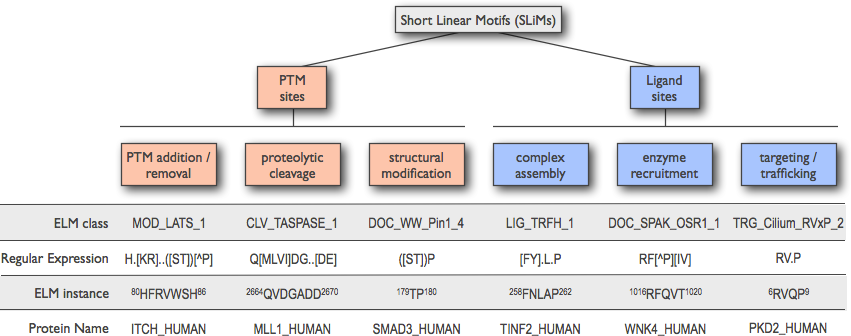
\includegraphics[width=\textwidth]{Figures/functional_classification_of_SLiMs.png}
\caption{
\textbf{Figure functional\_classification\_of\_SLiMs} For each ELM
class, the functional category to which it belongs is indicated by a
three-letter prefix. Each ELM class is defined by a regular expression.
Peptide sequences in proteins that match the regular expression of a
specific ELM class and that were experimentally validated to be
functional motifs are captured as ELM instances of that class. Degrons
are a specific subtype of enzyme-recruiting docking motifs (see text for
a detailed description).
}
\end{figure}

\subsection{Critical Parameters and
Troubleshooting}\label{critical-parameters-and-troubleshooting}

\emph{instructions: optionally 2 separate sections.}

\section{Internet Resources with
Annotations}\label{internet-resources-with-annotations}

http://www.clustal.org/omega Clustal Omega (\cite{21988835}) is a tool
for the alignment of multiple nucleic acid and protein sequences.

http://www.jalview.org Jalview (\cite{19151095}) is a Java desktop
application (and browser applet) that employs web services for sequence
alignment and visualization.

http://proviz.ucd.ie ProViz (\cite{27085803}) is an interactive protein
exploration tool, which searches several databases for information about
a given query protein. Data relevant to the protein like an alignment of
homologues, linear motifs, post translational modifications, domains,
secondary structure, sequence variations and others are graphically
represented relative to their position in the protein.
